%%% Wähle zwischen 16:9 und 4:3 Format
\documentclass[aspectratio=169]{beamer} % 16:9
% \documentclass{beamer} % 4:3

\usepackage[ngerman]{babel} % Deutsche Sprache
\usepackage[utf8]{inputenc}
\usepackage{tikz}
\usepackage{graphicx}
\usepackage{array}
\usepackage{booktabs}
\usepackage{amsmath}

\usetheme{aig}

\title{Stimmungsanalyse mit Twitter}
\author[Team Twitter Sentiment]{Anne Huber, Andreas Franke, Felix Lindner, Burak Özkan, Milomir Soknic}
\institute{Projektpraktikum Web Science,\\Artificial Intelligence Group,\\Universität Hagen, Deutschland}
\date{18. März 2025}

\begin{document}

% --- Titlepage ---
\begin{frame}
  \titlepage
\end{frame}

% --- Tweet-Folie ---
% \begin{frame}
%   \centering
%   
\includegraphics[width=\linewidth]{tweet.jpg}
% \end{frame}

\begin{frame}{Motivation}
  \begin{columns}
    % Linke Spalte: Bilder
    \column{0.5\textwidth}
    \centering
    
\includegraphics[scale=0.2]{Tweets.png}

    % Rechte Spalte: Stichpunkte zur Motivation
    \column{0.5\textwidth}
    \begin{itemize}
        \item Twitter als Echtzeit-Plattform für Meinungen und Trends
        \item Große Datenmengen für maschinelles Lernen nutzbar
        \item Herausforderungen: Ironie, Sarkasmus, Emojis, Abkürzungen
        \item Einsatz in Politik, Marketing und Krisenmanagement
    \end{itemize}
  \end{columns}
\end{frame}

\begin{frame}{Zielsetzung}
  \Large
  \begin{itemize}
      \item Wie effektiv sind verschiedene maschinelle Lernverfahren bei der Stimmungsanalyse von Tweets?
  \end{itemize}
\end{frame}

%=========================================================================================================================
\section{Daten}

\subsection{Datenauswahl}
\begin{frame}{Datenauswahl}
  \begin{itemize}
      \item Prüfung diverser Datensätze
      \item Entscheidung für \glqq Sentiment140\grqq
      \item Besonderheiten:
      \begin{itemize}
          \item Emojis als Sentiment-Indikatoren
          \item Ausbalancierte Klassen
          \item Bessere Datenqualität
          \item Artikel: \glqq Twitter Sentiment Classification using Distant Supervision\grqq
      \end{itemize}

      \vspace{0.5cm}
  \textbf{Beispieltweet:}
  \vspace{0.2cm}

  % Umwandlung mit Emoji => Tweet aus Datensatz
\begin{figure}
    \centering
    \begin{columns}[T]
        % Original Tweet Column
        \begin{column}{0.45\textwidth}
            \centering
            \textbf{Original Tweet}\\
            \textit{Just got my dream job! So excited! \yellowhighlight{:)}}
            \vspace{0.5cm}
        \end{column}

        % Arrow
        \begin{column}{0.1\textwidth}
            \centering
            \LARGE $\Rightarrow$
        \end{column}

        % Processed Tweet Column
        \begin{column}{0.45\textwidth}
            \centering
            \textbf{Datensatz}\\
            \textit{Just got my dream job! So excited!} \\
            \vspace{0.2cm}
            \textbf{Sentiment: \yellowhighlight{Positive}}
            \vspace{0.5cm}
        \end{column}
    \end{columns}
\end{figure}

  \end{itemize}
\end{frame}

\subsection{Testdatensatz}
\begin{frame}{Testdatensatz}
  \textbf{Eigenschaften:}
  \begin{itemize}
      \item Enthält \textbf{359} manuell gesammelte Tweets
      \item \textbf{177} negative und \textbf{182} positive Tweets
      \item Keine automatische Emoticon-Tagging-Strategie (bessere Qualität)
      \item Dient zur unabhängigen Evaluierung von Modellen
      \item Testdatensatz enthält zusätzlich \textit{Query-Terms}
  \end{itemize}

  \vspace{0.5cm}
  \textbf{Beispieltweet:}


  % Anstelle von positiven und negativen Tweets, Besipiele aus Testdatensatz mit Query-Term
  \begin{center}
    \glqq \textit{no. it is too big. I'm quite happy with the \yellowhighlight{Kindle2}\grqq}
    \vspace{0.25cm}
    \begin{columns}
        \begin{column}{0.45\textwidth}
            \textbf{Ohne Query Term: \darkhighlight{Negative}}
        \end{column}
        \begin{column}{0.45\textwidth}
            \textbf{Mit Query Term: \darkhighlight{Positive}}
        \end{column}
    \end{columns}
  \end{center}
\end{frame}



%=========================================================================================================================
\section{Klassische Methoden}

\subsection{Datenvorverarbeitung}

% Überschrift anpassen?
% Merkmassextraktion passt ggf. nicht zur Aufbereitung der Daten.
\begin{frame}{Datenvorverarbeitung}
  \fontsize{10pt}{12pt}\selectfont
  \vspace{0.3cm}

 \begin{table}[]
      \centering
      \renewcommand{\arraystretch}{1.2}
      \begin{tabular}{l|p{7.5cm}}
          \hline
          & \textbf{Beispiel (Sentiment140)} \\
          \hline
          \textbf{Original-Tweet} & \texttt{'@user I love this movie! :) http://example.com'} \\
          \hline
          \textbf{Bereinigung} & \texttt{'I love this movie'} \\
          \hline
          \textbf{Tokenisierung} & \texttt{['I', 'love', 'this', 'movie']} \\
          \hline
          \textbf{Transformation} & Lemmatization: \texttt{['I', 'love', 'this', 'movie']} \newline
          Stemming: \texttt{['I', 'lov', 'thi', 'movi']} \\
          \hline
          \textbf{Stopword-Handling} & Ohne Stoppwörter: \texttt{['love', 'movie']} \\
          \hline
          \textbf{Merkmalsextraktion} & TF-IDF Beispiel: \newline
          \texttt{(love: 0.75, movie: 0.85)} \\
          \hline
      \end{tabular}
  \end{table}

\end{frame}

\subsection{Klassische Methoden}

\begin{frame}{Klassische Methoden}
  \fontsize{10pt}{12pt}\selectfont
  \vspace{0.3cm}

  \begin{columns}
      % Linke Spalte: Methoden
      \column{0.45\textwidth}
      \textbf{Klassische Methoden}
      \vspace{0.3cm}
      \begin{itemize}
          \item \textbf{Logistische Regression}
          \item \textbf{\textit{Support Vector Machine (SVM)}}
          \item \textbf{Naiver Bayes}
          \item \textcolor{gray}{Entscheidungsbäume}
          \item \textcolor{gray}{Random Forests}
          \item \textcolor{gray}{K-nächste Nachbarn}
      \end{itemize}
      \vspace{0.5cm}
  \textbf{Metrik:} Genauigkeit
    \vspace{-0.5cm}
      % Rechte Spalte: Parameterarten
      \column{0.55\textwidth}
      \textbf{Parameter}
      \vspace{0.3cm}
      \begin{itemize}
    \item \texttt{Vektorisierungsmethode}
    \item \texttt{Normalisierungsstrategie}
    \item \texttt{Strategie zur Entfernung von Stoppwörtern}
    \item \texttt{N-Gramm-Bereich}
    \item \texttt{Maximale Anzahl an Merkmalen}
    \item \texttt{Anzahl der verwendeten Rechenkerne}
\end{itemize}
  \end{columns}
\end{frame}

% - Text Accuracy in Genauigkeit umändern
% - Balken der Größe nach anordnen
% - Anmerkung zu gekürzter Y-Achse | Y-Achse nicht kürzen?

\begin{frame}{Ergebnisse - Beste Genauigkeit pro Modell}
    \centering
    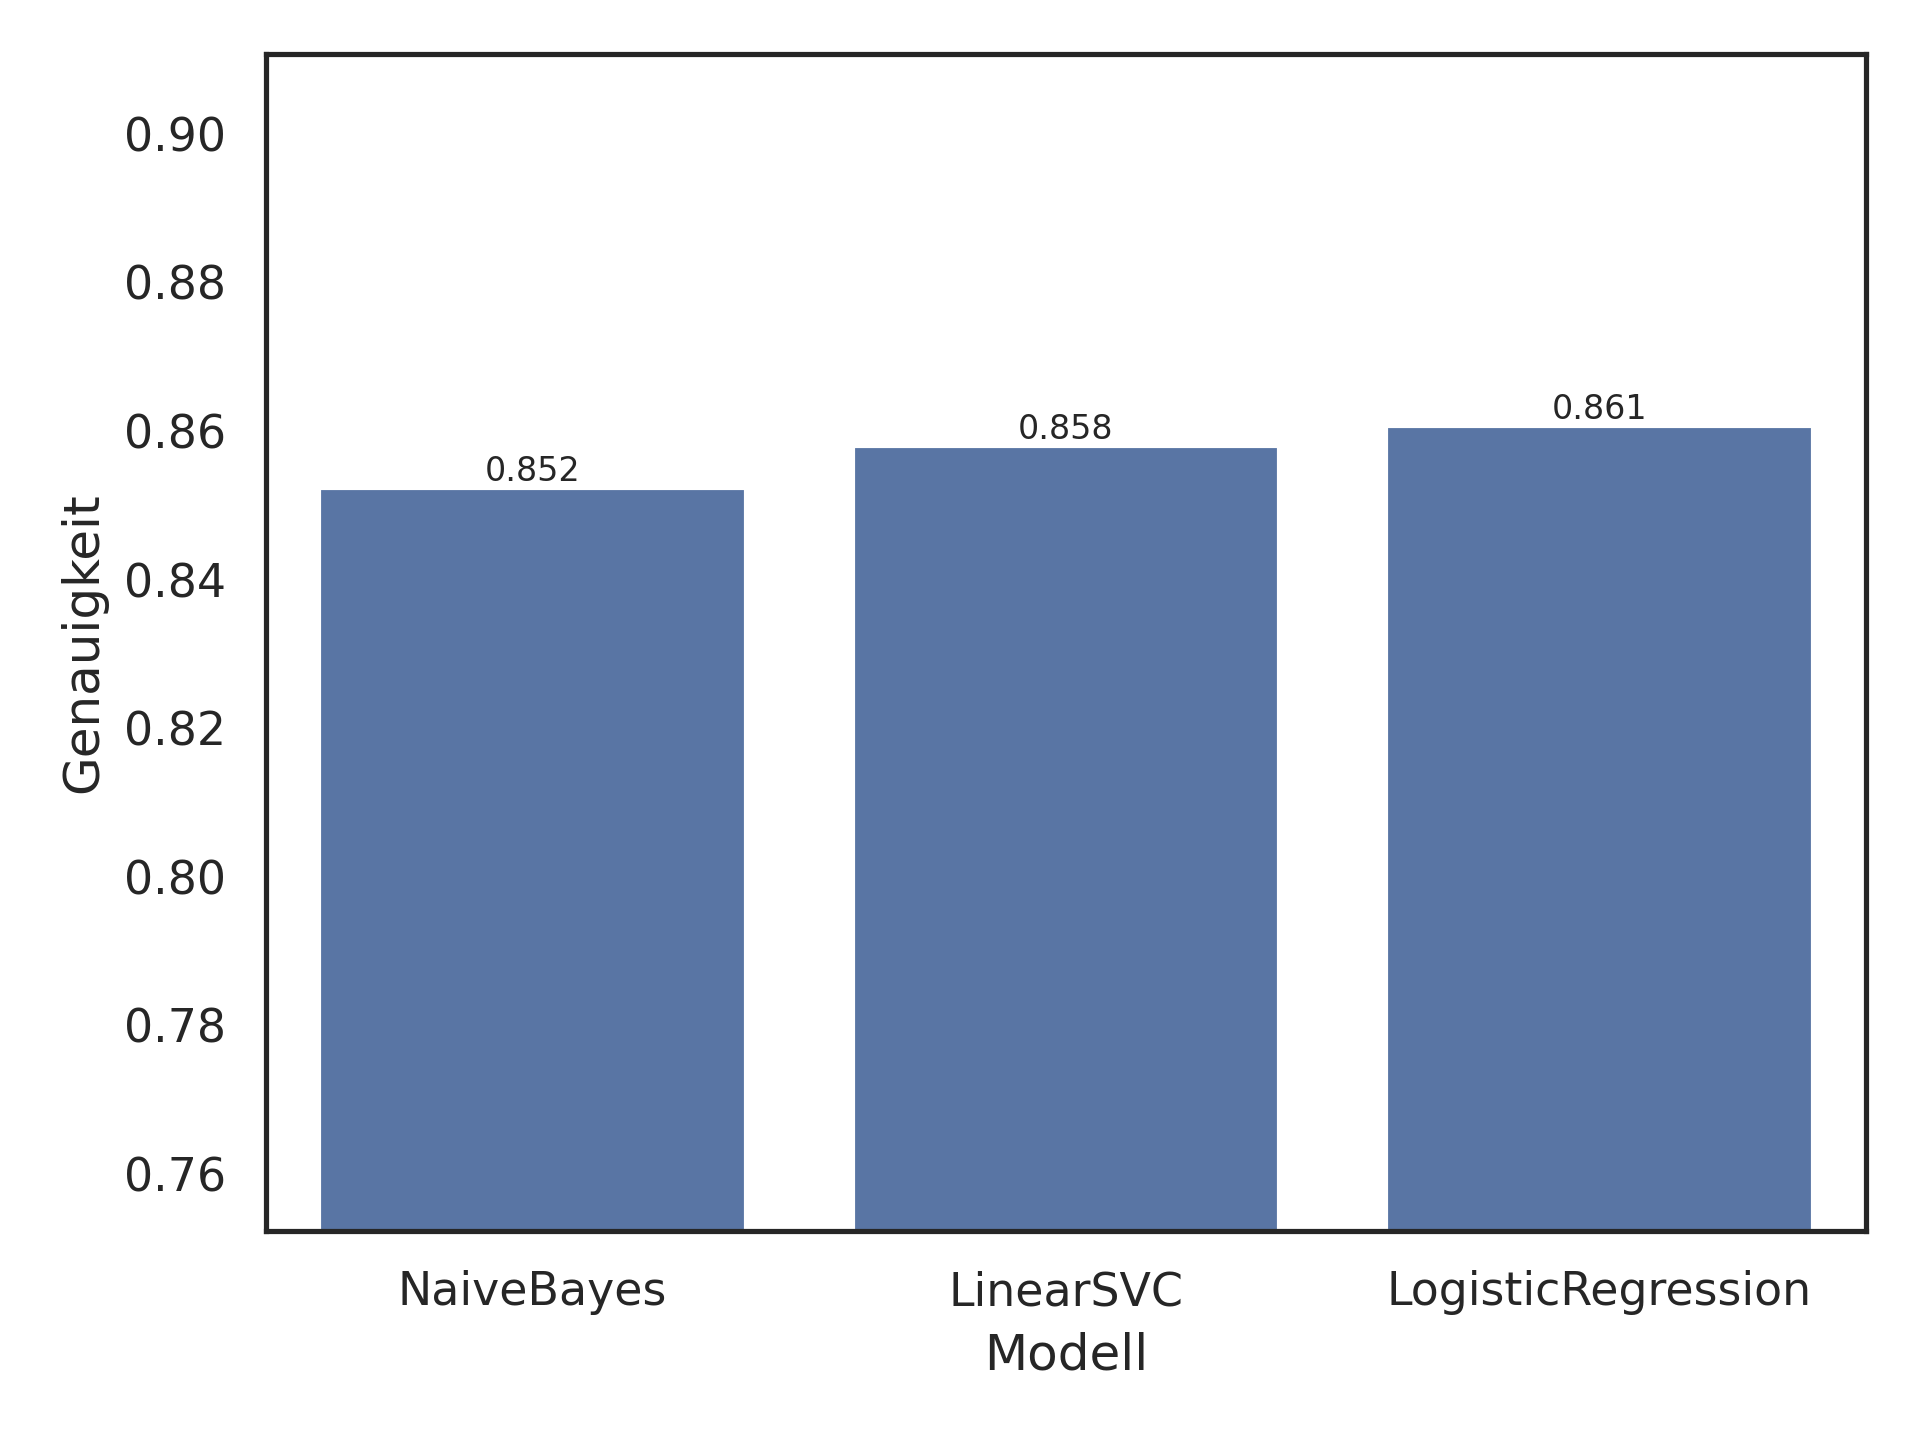
\includegraphics[scale=0.65]{../datasets/sentiment140/results/plots/klassische-ml-beste-genauigkeit-pro-modell-truncated-y-axis.png}
\end{frame}

% \begin{frame}{Ergebnisse}
%     \centering
%     \scriptsize
%     % Tabelle durch Box-Plots ersetzen
%     % Gegebenenfalls auf top-k und bottom-k Parameterkombinationen beschränken

%     % Diagrammtypen ausprobieren
%     % - Box-Plot
%     % - Balkendiagramm
%     % - Heatmap

%     \begin{tabular}{|l|l|l|l|l|}
%         \hline
%         \textbf{Modell} & \textbf{Vektorisierer} & \textbf{Max Features} & \textbf{N-Gram Range} & \textbf{Test Accuracy} \\
%         \hline
%         Log. Regression & TfidfVectorizer & 250000 & Uni- und Bigramme & 0.8607 \\
%         SVM & TfidfVectorizer & Alle Features & Uni-, Bi- und Trigramme & 0.8579 \\
%         Naiver Bayes & TfidfVectorizer & Alle Features & Uni- und Bigramme & 0.8524 \\
%         \hline
%     \end{tabular}
% \end{frame}


%=========================================================================================================================
\section{Deep Learning}

\subsection{Bert-Modelle}
% \begin{frame}{Twitter roberta-base-sentiment}
% \begin{itemize}
%       \item BERT-basiert
%       \item vortrainiert ohne unseren Datensatz
%       \item mit Testdatensatz evaluiert
%       \vspace{0.5cm}
%       \item \textbf{Genauigkeit:} 0,87
%   \end{itemize}
% \end{frame}

\begin{frame}{BERT}
    \begin{itemize}
        \item 2018 von Google entwickelt
        \item Bidirectional encoder representations from transformers (BERT)
        \item LLM
        \item Encoder
    \end{itemize}
\end{frame}

% 100M Parameter
\begin{frame}{Untersuchte BERT-Modelle}
\begin{columns}[T]
    \column{0.5\textwidth}
    \begin{block}{DistilBERT-base-uncased}
    \begin{itemize}
    \item Destilliertes BERT-Modell
    \item \textbf{Eigenschaften}:
      \begin{itemize}
      \item Modelldestillation des bert-base-uncased Modells
      \item 40\% kleiner
      \item 60\% schnellere Inferenz
      \item 97\% der Fähigkeiten bleiben erhalten
      \end{itemize}
    \end{itemize}
    \vspace{0.04cm}
    \end{block}
    \column{0.5\textwidth}
    \begin{block}{Twitter-RoBERTa-base-sentiment}
        \begin{itemize}
        \item Auf Twitter-Daten trainiertes RoBERTa-Modell
        \item \textbf{Eigenschaften}:
          \begin{itemize}
          \item Mit 58M englischsprachigen Tweets weitertrainiert
          \item Fine-Tuned mit einem Stimmungsanalyse-Datensatz
          \end{itemize}
        \end{itemize}
        \vfill
    \end{block}
\end{columns}
\end{frame}

\subsection{Fine-Tuning BERT-Modelle}

\begin{frame}{Fine-Tuning BERT-Modelle}
\begin{itemize}
        \item \textbf{Methode}
            \begin{itemize}
                \item Huggingface \textit{transformers} Bibliothek
            \end{itemize}
        \item \textbf{Untersuchte Parameter:}
        \begin{itemize}
            \item Initiale Lernrate
            \item Größe des Trainingsdatensatzes
        \end{itemize}
        \item \textbf{Evaluationsmetrik:}
        \begin{itemize}
            \item Genauigkeit
        \end{itemize}
\end{itemize}
\end{frame}

% \begin{frame}{Ergebnisse}
%     \centering
%     \scriptsize
%     \begin{tabular}{|l|l|l|l|}
%         \hline
%         \textbf{Modell} & \textbf{Daten-Größe} & \textbf{Lernrate} & \textbf{Test Accuracy} \\
%         \hline
%         DistilBERT & 20.000 & 0.0001 & 0.8496 \\
%         RoBerta-Twitter & 20.000 & 0.0001 & 0.9220 \\
%         \hline
%     \end{tabular}
% \end{frame}

\begin{frame}{Ergebnisse - BERT-Modelle}
    \centering
     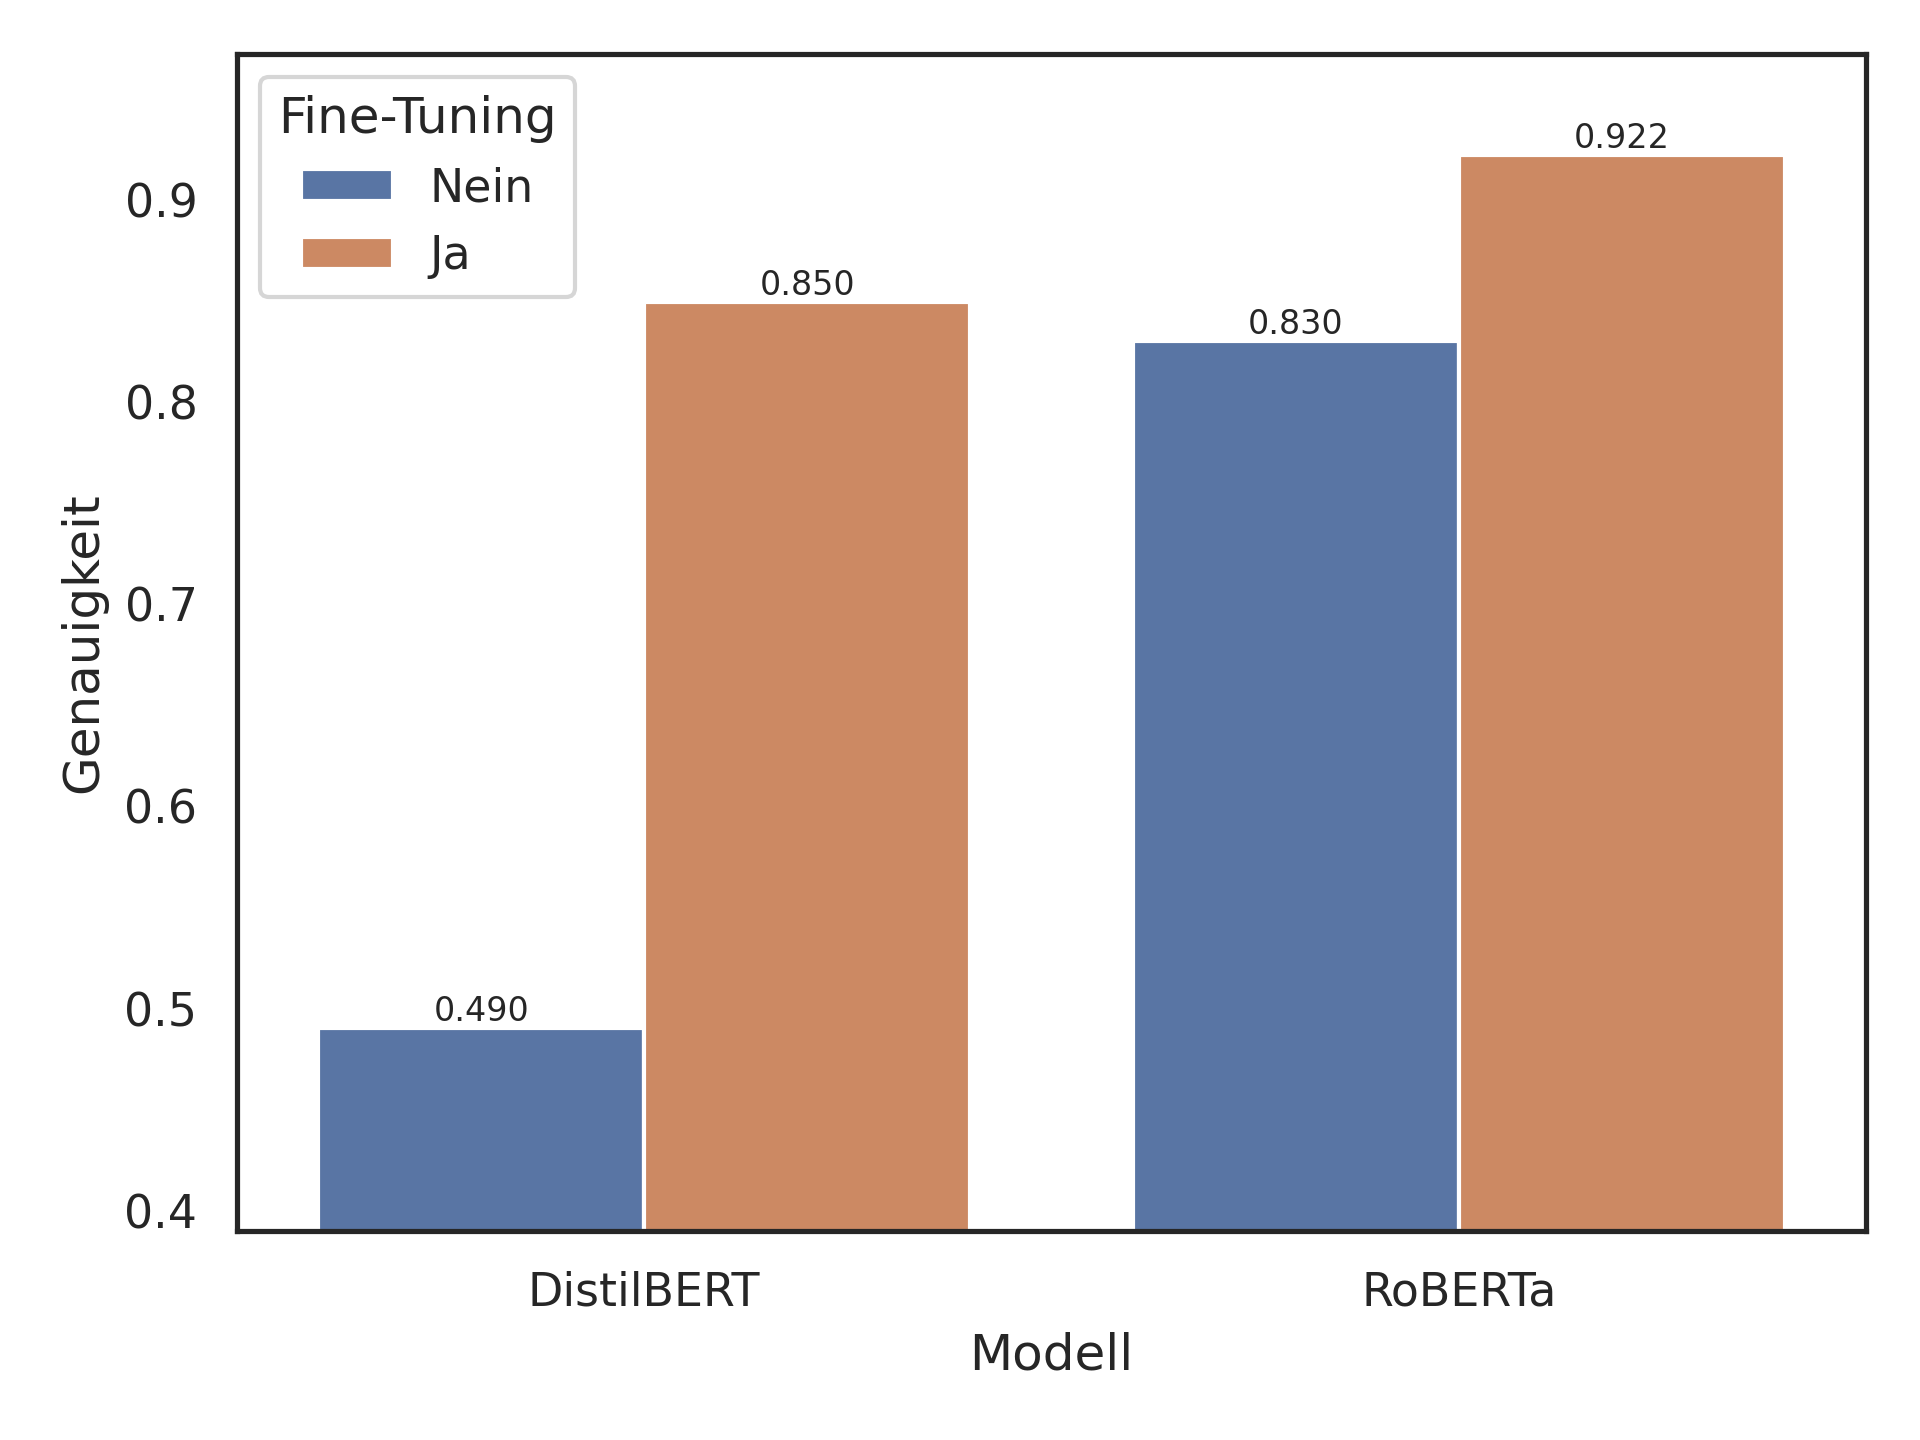
\includegraphics[scale=0.65]{../datasets/sentiment140/results/plots/bert-based-genauigkeit-bert-basierte-modelle-default-vs.-fine-tuned-truncated-y-axis.png}
\end{frame}

% BERT-basiert Modelle

% Erläuterung BERT-Modelle
% Fine-Tuning Ansatz
% Verwendet Modelle + Parameter
% Ergebnisse (jeweils ohne Fine-Tuning/Zero-Shot + Fine-Tuning)



% DeepSeek R1

% Modell-Erläuterung
% Fine-Tuning Ansatz lediglich erwähnen
% Verwendet Modelle + Prompt
% Ergebnisse (mit/ohne token-basierten Ansatz)
%  + Reasoning-Output

\subsection{DeepSeek}

\begin{frame}{DeepSeek-R1}
\begin{itemize}
\item \textbf{Reasoning-Modell}
\item Basiert auf Transformer Architektur
\item Trainiert mit Hilfe von Reinforcement Learning
\item 671 Mrd. Parameter
\item Destillierte Modelle verfügbar
\end{itemize}
\vspace{0.4cm}

\begin{itemize}
    \item \textbf{Fine-Tuning Ansatz}
    \begin{itemize}
        \item \textit{DeepSeek-R1-Distill-Qwen-1.5B}
        \item Aufgrund von Hardwareanforderungen verworfen
\end{itemize}
\end{itemize}
\end{frame}

\begin{frame}{Zero-shot}
  \textbf{Zero-Shot-Ansatz:}

  \vspace{0.35cm}

  \begin{itemize}
      \item Prompt enthält keine Beispiele
      \item Verwendete Modelle
      \begin{itemize}
          \item DeepSeek-1.5B
          \item DeepSeek-8B
          \item DeepSeek-32B
          \item DeepSeek-70B
      \end{itemize}
      \item Inferenz mit und ohne Query-Terms
  \end{itemize}
  \vspace{0.2cm}
  \centering
  \textbf{Prompt:} Tweet sentiment? Sentiment Topic: \{Query-Term\} \\
  Answer with positive or negative. Provide reasoning in JSON.\\
    Tweet: \glqq\{tweet\}\grqq
\end{frame}

\begin{frame}{Beispiel}
\begin{center}
    \textbf{Tweet:} \glqq \textit{no. it is too big. I'm quite happy with the \yellowhighlight{Kindle2}\grqq}
    \vspace{0.45cm}
    \begin{columns}
        \begin{column}{0.45\textwidth}
            \textbf{Reasoning ohne Query Term} \\
            \vspace{0.4cm}
            \glqq \textit{The tweet expresses dissatisfaction with something being 'too big,' indicating a \darkhighlight{negative sentiment}.\grqq}
        \end{column}
        \begin{column}{0.45\textwidth}
            \textbf{Reasoning mit Query Term:} \\
            \vspace{0.4cm}
            \glqq \textit{The tweet mentions being 'quite happy' with the Kindle2, which indicates a \darkhighlight{positive sentiment}.\grqq}
        \end{column}
    \end{columns}
\end{center}

\end{frame}

%distilbert-base-uncased


\begin{frame}{Ergebnisse - DeepSeek-Modelle mit/ohne Query-Term}
    \centering
    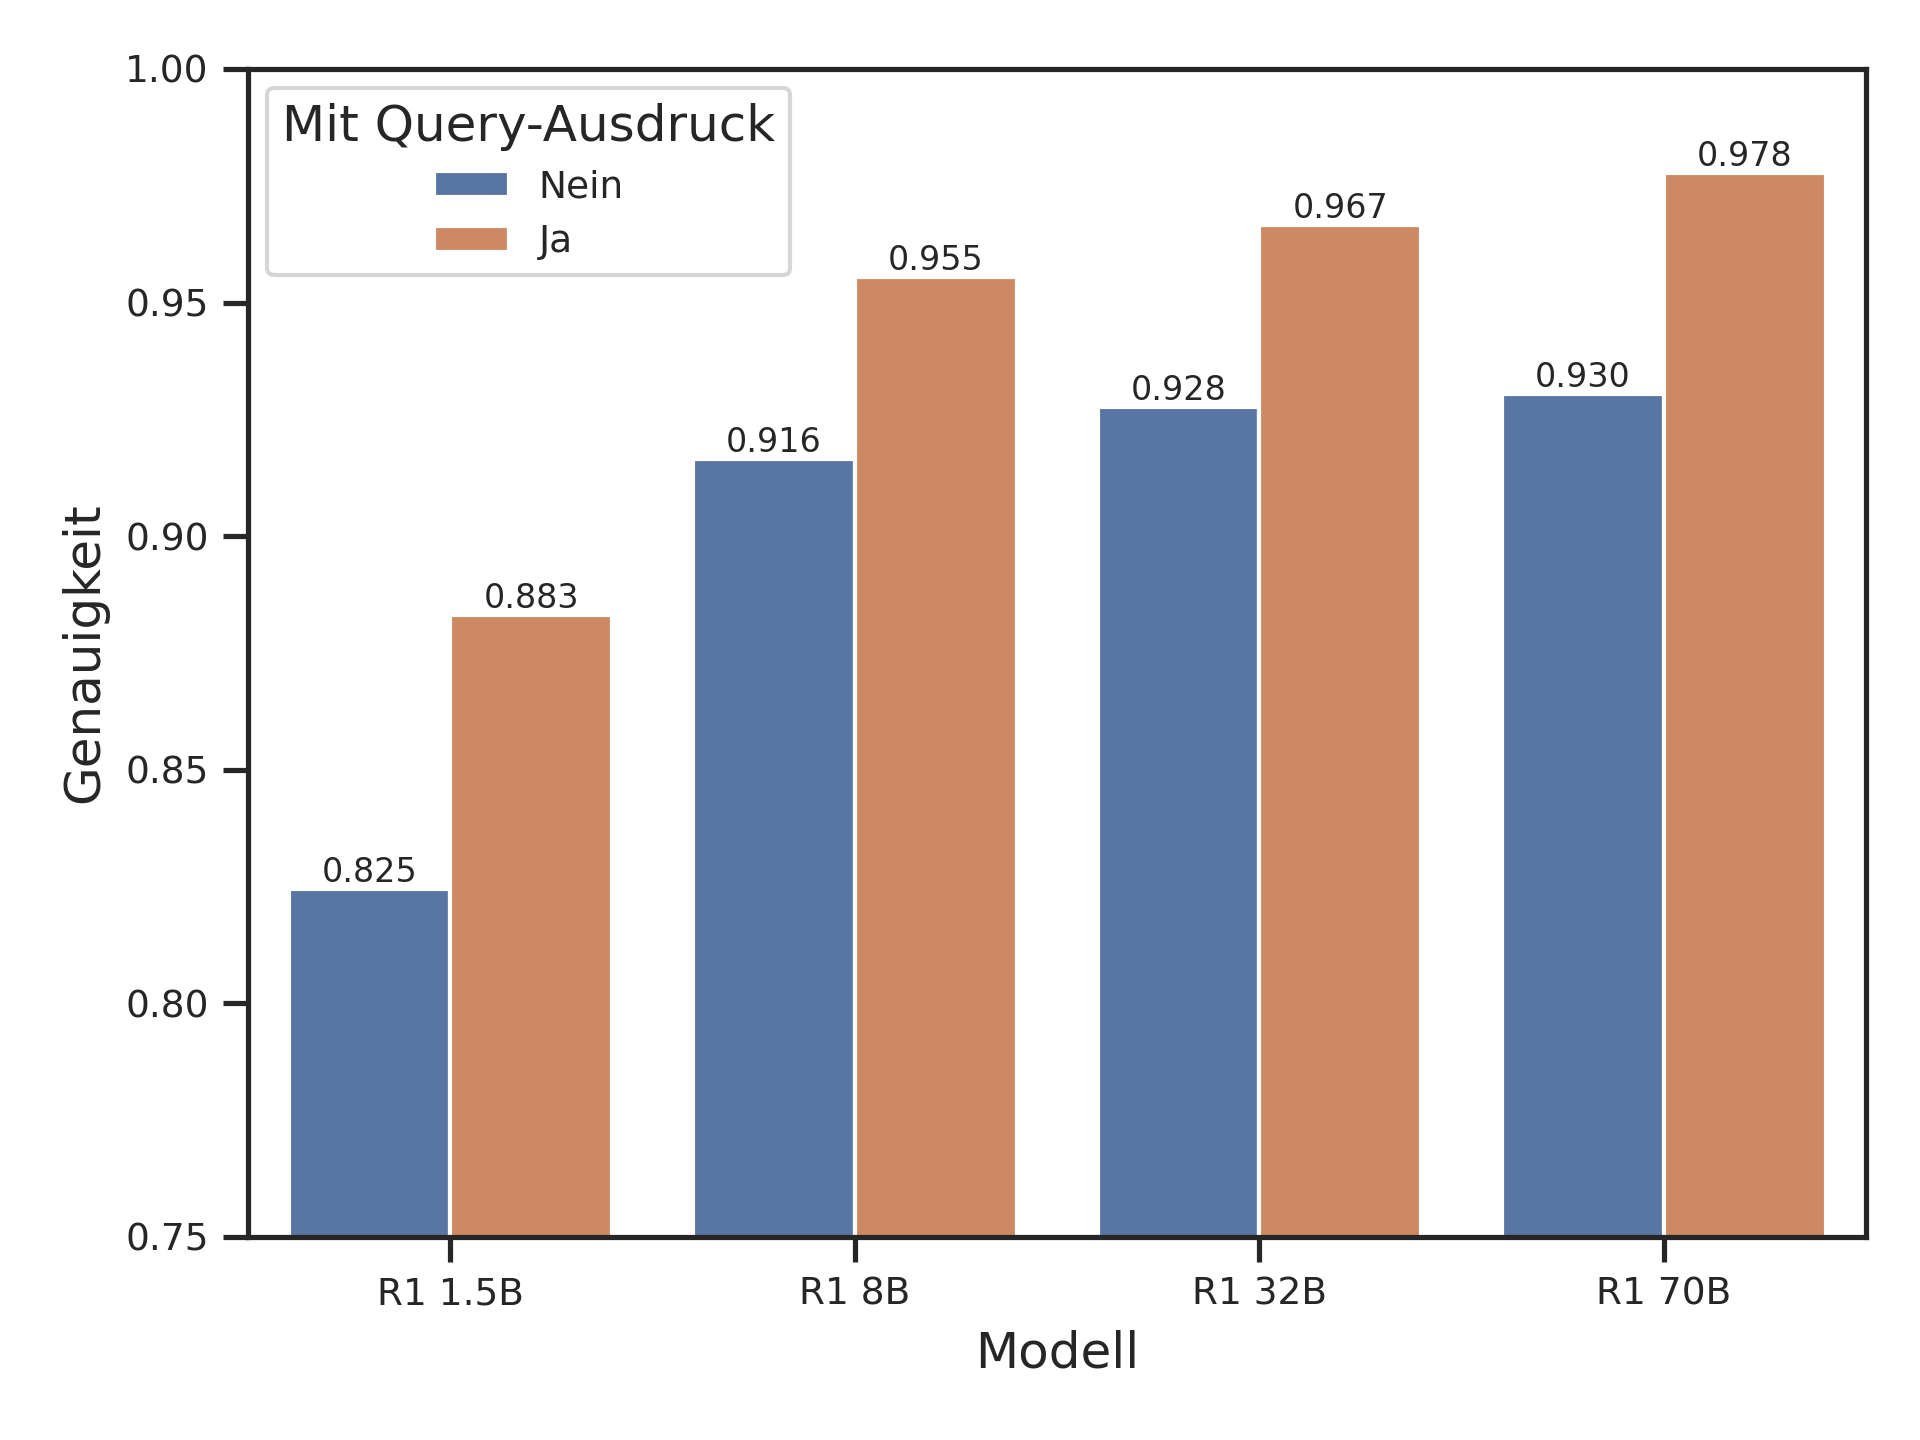
\includegraphics[scale=0.65]{../datasets/sentiment140/results/plots/deepseek-genauigkeit-deepseek-modelle-einfluss-query-ausdruck-truncated-y-axis.png}
\end{frame}

% \begin{frame}{Ergebnisse: BERT- und DeepSeek-Modelle}
%     \centering
%     \scriptsize
%     \begin{tabular}{|l|l|l|l|}
%         \hline
%         \textbf{Modell} & \textbf{Daten-Größe} & \textbf{Lernrate} & \textbf{Test Accuracy} \\
%         \hline
%         DistilBERT & 20.000 & 0.0001 & 0.8496 \\
%         RoBerta-Twitter & 20.000 & 0.0001 & 0.9220 \\
%         DeepSeek & 20.000 & 0.0001 & 0.8663 \\
%         \hline
%     \end{tabular}
% \end{frame}

% Prompt Options???

% \begin{frame}{Ergebnisse}
%     \centering
%     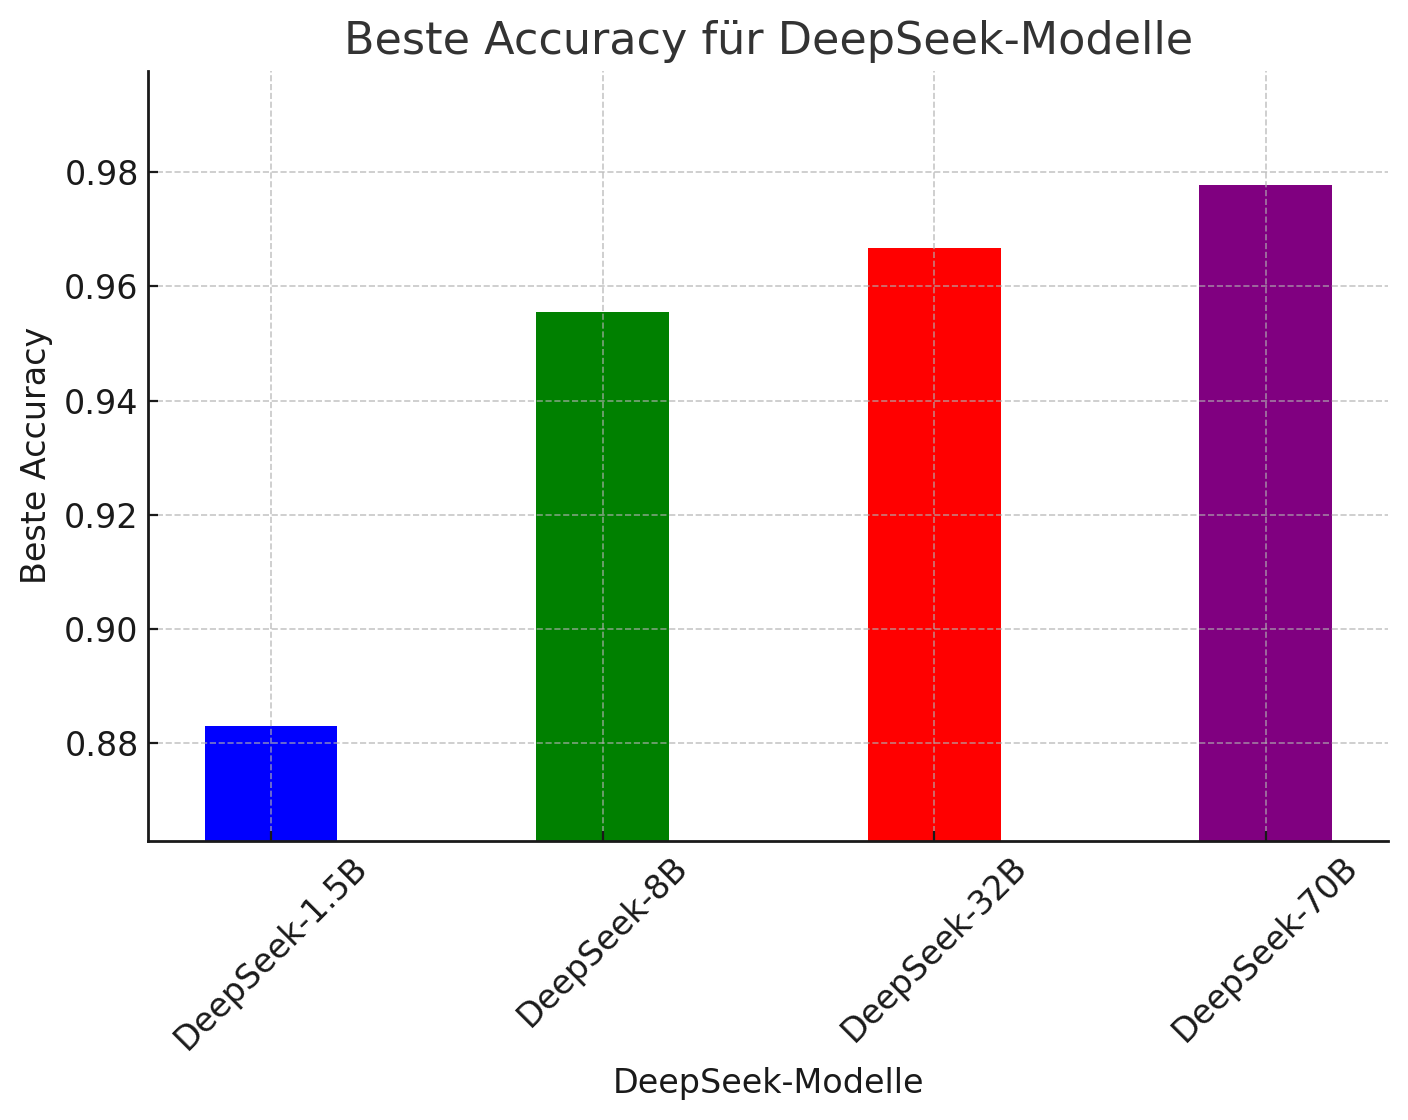
\includegraphics[scale=0.3]{deepseekzero.png}
% \end{frame}

% \begin{frame}{Ergebnisse}
%     \centering
%     \scriptsize
%     \begin{tabular}{|l|l|l|}
%         \hline
%         \textbf{Modell} & \textbf{Mit Query-Term} & \textbf{Ohne Query-Term} \\
%         \hline
%         DeepSeek-1.5B & 0.8830 & 0.8245 \\
%         DeepSeek-8B   & 0.9554 & 0.9164 \\
%         DeepSeek-32B  & 0.9666 & 0.9276 \\
%         DeepSeek-70B  & 0.9777 & 0.9304 \\
%         \hline
%     \end{tabular}
% \end{frame}



%=========================================================================================================================
\section{Zusammenfassung}

\begin{frame}{Zusammenfassung - Überblick Ergebnisse alle Modelle}
    \centering
    \includegraphics[scale=0.65]{../datasets/sentiment140/results/plots/alle-übersicht-genauigkeit-alle-modelle-truncated-y-axis.png}
\end{frame}

% Stärkerer Fokus auf Ergebnisse
% - Vergleich der Modelle / Übersichts-Diagramm
% - Einschränkungen der einzelnen Modelle (Hardware, Trainingszeit)
\begin{frame}{Zusammenfassung}
  \normalsize
  % \begin{itemize}
  %     \item Stimmungsanalyse auf dem Sentiment140-Datensatz
  %     \item Klassische Methoden
  %     \item BERT-Modelle Fine-Tuning
  %     \item Zero-Shot-Ansatz für destillierte DeepSeek-Modelle
  %     \pause
  %     \end{itemize}
      \begin{itemize}
        \item \textbf{Erkenntnisse:}
        \begin{itemize}
            \item Domänenspezifische Transformer Modelle besser als allgemeine Modelle
            \item Query-Terms erhöhen die Genauigkeit für LLMs erheblich
            \item LLMs haben viel größere Hardwareanforderungen und längere Inferenzzeiten
        \end{itemize}
        \vspace{0.4cm}
        \item \textbf{Ausblick:}
        \begin{itemize}
            \item Noisy-Label
            \item Aspect-Based-Sentiment-Analysis (ABSA)
            \item Große Deep Learning Modelle
        \end{itemize}
    \end{itemize}

  \vspace{0.5cm}
  \centering
  \pause
  {\large \textbf{Vielen Dank für Ihre Aufmerksamkeit!}} \\[0.1cm]
  \textit{Fragen?}
\end{frame}

\end{document}
